\documentclass[11pt,letterpaper]{article}
\usepackage[utf8x]{inputenc}
\usepackage[T1]{fontenc}
\usepackage{amsmath}
\usepackage{amssymb}
\usepackage{graphicx}
\graphicspath{{../img/}}
\usepackage[spanish]{babel}

\title{Simulación Estocástica - Taller 2}
\author{Jesid Mauricio Mejía Castro}

\begin{document}
	\maketitle
	
	\section{Deteniendo la simulación de datos}	
	\begin{itemize}
		\item[a)] Dado que se requiere que $n \geq 100$ y $S/\sqrt{n} < 0.01$. Al despejar $n$ de la desigualdad tendremos que:
		\[ 100 \leq n < 10000S^2 \text{.} \]
		Al tratarse de una variable aleatoria normal estándar, sabemos que $S = 1$, por tanto se espera que el valor de $n$ sea cercano a $10000$.
		\item[b)] Con el código en R (véase el archivo {\ttfamily p1.R}) se obtiene un valor de $n=9897$.
		\item[c)] La media de la muestra fue $\bar{X}=-0.01482648$.
		\item[d)] La varianza de la muestra fue $S^2=0.9974088$.
		\item[e)] Los resultados obtenido eran de esperarse pues estamos tratando con una variable aleatoria normal estándar, es decir, $\mu=0$ y $\sigma^2=1$.
	\end{itemize}

	\newpage

	\section{Intervalos de confianza}
	El código ({\ttfamily p2.R}) genera la siguiente salida para 15 pruebas y 100 variables $U(-1,1)$:
	
	\begin{verbatim}
		Number of trials: 15
		
		sample mean  lower bound   upper bound  contains mean?
		-0.01774    -0.05520       +0.01971     1
		-0.02129    -0.05874       +0.01617     1
		-0.03336    -0.07081       +0.00410     1
		+0.01779    -0.01966       +0.05525     1
		-0.03178    -0.06924       +0.00567     1
		-0.03436    -0.07181       +0.00310     1
		-0.01445    -0.05191       +0.02300     1
		+0.01570    -0.02176       +0.05315     1
		-0.01503    -0.05249       +0.02242     1
		-0.00332    -0.04077       +0.03414     1
		+0.01621    -0.02124       +0.05366     1
		-0.00902    -0.04648       +0.02843     1
		+0.01184    -0.02561       +0.04929     1
		+0.00867    -0.02879       +0.04612     1
		+0.01459    -0.02286       +0.05205     1
		
		100 per cent of CI's contain the mean.
	\end{verbatim}

	\section{\textit{Bootstrap}}
	
	\begin{itemize}
		\item[a)] La distribución de la desviación estándar puede verse en la Figura \ref{fig:p3a}.
		\item[b)] $E[S] = 0.4595913$.
		\item[c)] $\hat{q}_{0.5} = 1.300492$.
		\item[c)] $ \text{Var}[S] = 0.2112242$.
		\begin{figure}[h]
			\centering
			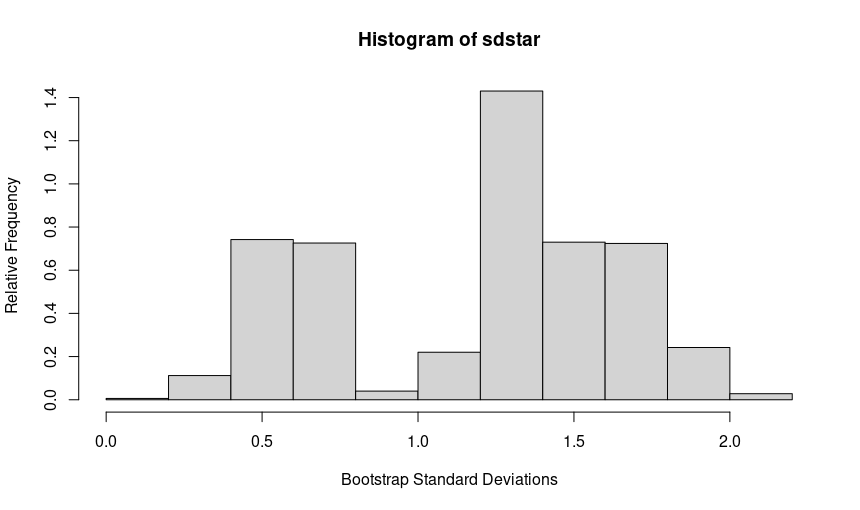
\includegraphics[width=0.7\linewidth]{../img/p3_a}
			\caption{Distribución de las desviaciones estándar para $y*$.}
			\label{fig:p3a}
		\end{figure}
		
	\end{itemize}

	\section{Simulación de dos dados}
	
	\begin{itemize}
		\item[a)] En el código fuente del archivo {\ttfamily p4.R} puede encontrarse la función que simula el lanzamiento de dos dados. La idea de la simulación es aproximar dos números aleatorios distribuidos con $U(1, 7)$ al menor entero más cercano (la función piso). Es decir:
		
		\[
		x_i = \lfloor U(1, 7) \rfloor\ \text{para}\ i=1,2\text{.}
		\]
		
		De manera que $M = \min(x_1, x_2)$.
		\item[b)] Con $n = 10^4$ simulaciones, se obtuvo que el valor esperado es $E[M] = 2.54490$, la varianza $V(M) = 1.93897$. Además, se obtuvo que la probabilidad $P(M \geq 3) = 0.4471$.
		\item[c)] Con una confianza del 95\% se tiene que la media está contenida en el intervalo $[2.53248, 2.58812]$.
		\item[d)] La media y su intervalo de confianza al 95\% puede verse en la Figura \ref{fig:p5d}. Se puede observar la estabilización alrededor el valor esperado.
		
		\begin{figure}[t!]
			\centering
			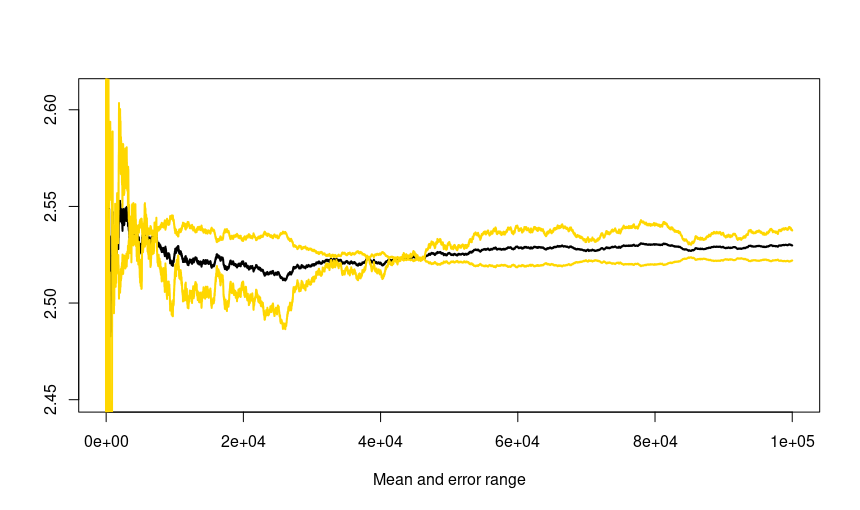
\includegraphics[width=0.7\linewidth]{../img/p5d}
			\caption{Intervalo de 95\% para la media con $10^5$ simulaciones de $M$.}
			\label{fig:p5d}
		\end{figure}
		
	\end{itemize}
	

	
\end{document}
